% This file was created with tikzplotlib v0.10.1.
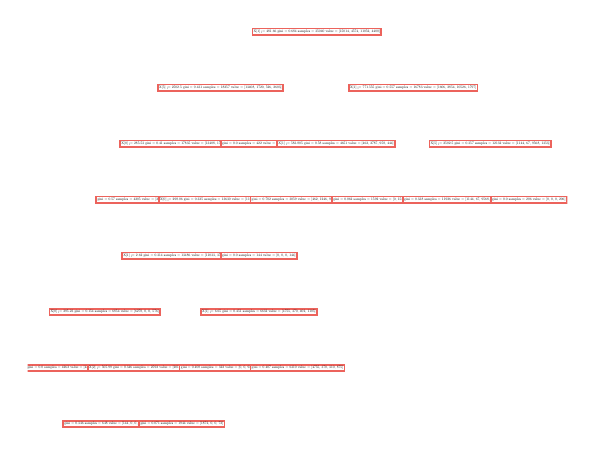
\begin{tikzpicture}

\definecolor{darkgray176}{RGB}{176,176,176}
\definecolor{tomato2369992}{RGB}{236,99,92}

\begin{axis}[
hide x axis,
hide y axis,
tick align=outside,
tick pos=left,
x grid style={darkgray176},
xmin=0, xmax=1,
xtick style={color=black},
y grid style={darkgray176},
ymin=0, ymax=1,
ytick style={color=black}
]
\draw (axis cs:0.142857142857143,0.0625) node[
  scale=0.130016244214914,
  fill=white,
  draw=tomato2369992,
  line width=0.6pt,
  inner sep=3.6pt,
  text=black,
  rotate=0.0,
  align=center
]{gini = 0.346
samples = 648
value = [144, 0, 0, 504]};
\draw (axis cs:0.285714285714286,0.0625) node[
  scale=0.130016244214914,
  fill=white,
  draw=tomato2369992,
  line width=0.6pt,
  inner sep=3.6pt,
  text=black,
  rotate=0.0,
  align=center
]{gini = 0.071
samples = 1944
value = [1872, 0, 0, 72]};
\draw (axis cs:0.0714285714285714,0.1875) node[
  scale=0.130016244214914,
  fill=white,
  draw=tomato2369992,
  line width=0.6pt,
  inner sep=3.6pt,
  text=black,
  rotate=0.0,
  align=center
]{gini = 0.0
samples = 4262
value = [4262, 0, 0, 0]};
\draw (axis cs:0.214285714285714,0.1875) node[
  scale=0.130016244214914,
  fill=white,
  draw=tomato2369992,
  line width=0.6pt,
  inner sep=3.6pt,
  text=black,
  rotate=0.0,
  align=center
]{X[2] <= 505.99
gini = 0.346
samples = 2592
value = [2016, 0, 0, 576]};
\draw (axis cs:0.357142857142857,0.1875) node[
  scale=0.130016244214914,
  fill=white,
  draw=tomato2369992,
  line width=0.6pt,
  inner sep=3.6pt,
  text=black,
  rotate=0.0,
  align=center
]{gini = 0.408
samples = 322
value = [0, 0, 92, 230]};
\draw (axis cs:0.5,0.1875) node[
  scale=0.130016244214914,
  fill=white,
  draw=tomato2369992,
  line width=0.6pt,
  inner sep=3.6pt,
  text=black,
  rotate=0.0,
  align=center
]{gini = 0.407
samples = 6310
value = [4755, 370, 310, 875]};
\draw (axis cs:0.142857142857143,0.3125) node[
  scale=0.130016244214914,
  fill=white,
  draw=tomato2369992,
  line width=0.6pt,
  inner sep=3.6pt,
  text=black,
  rotate=0.0,
  align=center
]{X[0] <= 295.23
gini = 0.154
samples = 6854
value = [6278, 0, 0, 576]};
\draw (axis cs:0.428571428571429,0.3125) node[
  scale=0.130016244214914,
  fill=white,
  draw=tomato2369992,
  line width=0.6pt,
  inner sep=3.6pt,
  text=black,
  rotate=0.0,
  align=center
]{X[1] <= 6.65
gini = 0.451
samples = 6632
value = [4755, 370, 402, 1105]};
\draw (axis cs:0.285714285714286,0.4375) node[
  scale=0.130016244214914,
  fill=white,
  draw=tomato2369992,
  line width=0.6pt,
  inner sep=3.6pt,
  text=black,
  rotate=0.0,
  align=center
]{X[1] <= 2.62
gini = 0.314
samples = 13486
value = [11033, 370, 402, 1681]};
\draw (axis cs:0.428571428571429,0.4375) node[
  scale=0.130016244214914,
  fill=white,
  draw=tomato2369992,
  line width=0.6pt,
  inner sep=3.6pt,
  text=black,
  rotate=0.0,
  align=center
]{gini = 0.0
samples = 144
value = [0, 0, 0, 144]};
\draw (axis cs:0.214285714285714,0.5625) node[
  scale=0.130016244214914,
  fill=white,
  draw=tomato2369992,
  line width=0.6pt,
  inner sep=3.6pt,
  text=black,
  rotate=0.0,
  align=center
]{gini = 0.57
samples = 4205
value = [2375, 1350, 124, 356]};
\draw (axis cs:0.357142857142857,0.5625) node[
  scale=0.130016244214914,
  fill=white,
  draw=tomato2369992,
  line width=0.6pt,
  inner sep=3.6pt,
  text=black,
  rotate=0.0,
  align=center
]{X[0] <= 298.06
gini = 0.325
samples = 13630
value = [11033, 370, 402, 1825]};
\draw (axis cs:0.5,0.5625) node[
  scale=0.130016244214914,
  fill=white,
  draw=tomato2369992,
  line width=0.6pt,
  inner sep=3.6pt,
  text=black,
  rotate=0.0,
  align=center
]{gini = 0.702
samples = 3059
value = [462, 1246, 907, 444]};
\draw (axis cs:0.642857142857143,0.5625) node[
  scale=0.130016244214914,
  fill=white,
  draw=tomato2369992,
  line width=0.6pt,
  inner sep=3.6pt,
  text=black,
  rotate=0.0,
  align=center
]{gini = 0.062
samples = 1592
value = [0, 1541, 51, 0]};
\draw (axis cs:0.785714285714286,0.5625) node[
  scale=0.130016244214914,
  fill=white,
  draw=tomato2369992,
  line width=0.6pt,
  inner sep=3.6pt,
  text=black,
  rotate=0.0,
  align=center
]{gini = 0.338
samples = 11926
value = [1144, 67, 9568, 1147]};
\draw (axis cs:0.928571428571429,0.5625) node[
  scale=0.130016244214914,
  fill=white,
  draw=tomato2369992,
  line width=0.6pt,
  inner sep=3.6pt,
  text=black,
  rotate=0.0,
  align=center
]{gini = 0.0
samples = 206
value = [0, 0, 0, 206]};
\draw (axis cs:0.285714285714286,0.6875) node[
  scale=0.130016244214914,
  fill=white,
  draw=tomato2369992,
  line width=0.6pt,
  inner sep=3.6pt,
  text=black,
  rotate=0.0,
  align=center
]{X[0] <= 285.53
gini = 0.41
samples = 17835
value = [13408, 1720, 526, 2181]};
\draw (axis cs:0.428571428571429,0.6875) node[
  scale=0.130016244214914,
  fill=white,
  draw=tomato2369992,
  line width=0.6pt,
  inner sep=3.6pt,
  text=black,
  rotate=0.0,
  align=center
]{gini = 0.0
samples = 422
value = [0, 0, 0, 422]};
\draw (axis cs:0.571428571428571,0.6875) node[
  scale=0.130016244214914,
  fill=white,
  draw=tomato2369992,
  line width=0.6pt,
  inner sep=3.6pt,
  text=black,
  rotate=0.0,
  align=center
]{X[1] <= 583.805
gini = 0.58
samples = 4651
value = [462, 2787, 958, 444]};
\draw (axis cs:0.857142857142857,0.6875) node[
  scale=0.130016244214914,
  fill=white,
  draw=tomato2369992,
  line width=0.6pt,
  inner sep=3.6pt,
  text=black,
  rotate=0.0,
  align=center
]{X[5] <= 2502.5
gini = 0.357
samples = 12132
value = [1144, 67, 9568, 1353]};
\draw (axis cs:0.357142857142857,0.8125) node[
  scale=0.130016244214914,
  fill=white,
  draw=tomato2369992,
  line width=0.6pt,
  inner sep=3.6pt,
  text=black,
  rotate=0.0,
  align=center
]{X[5] <= 2502.5
gini = 0.431
samples = 18257
value = [13408, 1720, 526, 2603]};
\draw (axis cs:0.714285714285714,0.8125) node[
  scale=0.130016244214914,
  fill=white,
  draw=tomato2369992,
  line width=0.6pt,
  inner sep=3.6pt,
  text=black,
  rotate=0.0,
  align=center
]{X[1] <= 771.555
gini = 0.557
samples = 16783
value = [1606, 2854, 10526, 1797]};
\draw (axis cs:0.535714285714286,0.9375) node[
  scale=0.130016244214914,
  fill=white,
  draw=tomato2369992,
  line width=0.6pt,
  inner sep=3.6pt,
  text=black,
  rotate=0.0,
  align=center
]{X[1] <= 481.66
gini = 0.684
samples = 35040
value = [15014, 4574, 11052, 4400]};
\end{axis}

\end{tikzpicture}
